\setcounter{ExampleCounter}{1}
In 1804, Thomas Jefferson won the U.S. presidential election, edging out Charles C. Pinckney by 65,191 votes.  A little over 100 years later, in the 1908 election, William Howard Taft beat William Jennings Bryan by 1,269,356 votes.  The question is, who had a wider margin of victory?
\begin{center}
\begin{tabular}{c c c}
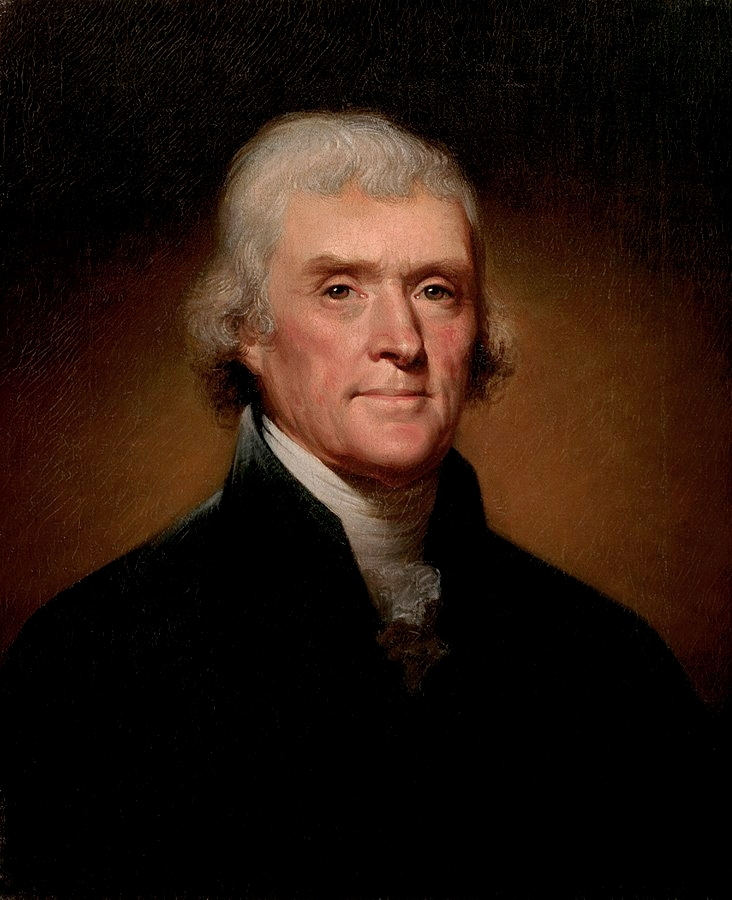
\includegraphics[height=2in]{ThomasJefferson} & \text{} \hspace*{1in} \text{} & 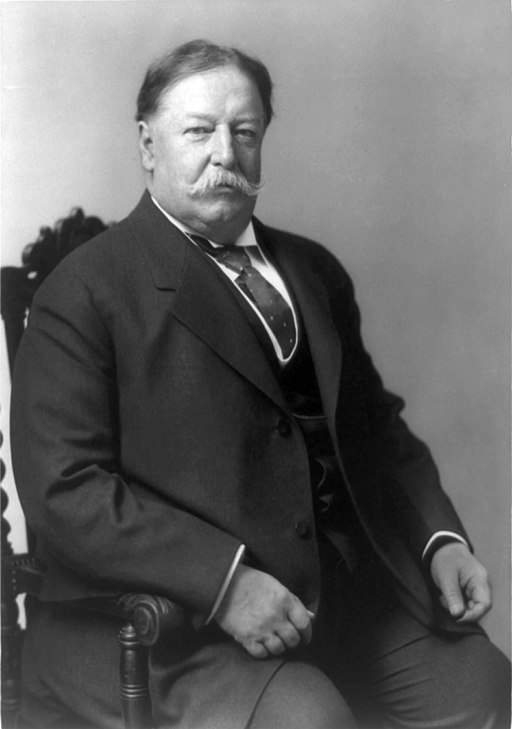
\includegraphics[height=2in]{WilliamTaft}\\
{\color{gray}Thomas Jefferson} & & {\color{gray}William Howard Taft}
\end{tabular}
\end{center}

Although Taft won his election by more votes than Jefferson, you've probably already spotted why this is misleading on its own: there were more votes cast in 1908 than in 1804.  In order to compare these two values fairly, we need more information; specifically, we need to know how many votes were counted in total each year.

There were only 143,029 total votes in 1804, compared to 14,889,239 in 1908.  Now all we need is a way to scale the margins of victory based on these totals; to do this, we can find what \textbf{percentage} of the total votes corresponds to the margin.

\paragraph{Jefferson} \[\dfrac{65,191}{143,029}=0.456=\scalebox{1.7}{45.6\%}\]

\paragraph{Taft} \[\dfrac{1,269,356}{14,889,239}=0.085=\scalebox{1.7}{8.5\%}\]

By putting both numbers in context, we can tell that Jefferson won by a historic margin; the \textit{difference} between him and his opponent was nearly half of all voters, and he won over 70\% of all votes.  Although Taft still won by a fairly large percentage, it was nowhere close to Jefferson's win.

\begin{formula}{Why Use Percentages?}
Percentages are used to add context to a number, and to scale numbers so that they can be compared.
\end{formula}
\pagebreak

It's often hard for us to put numbers--especially large numbers--in context, and percentages give us a consistent scale to work with.  For instance, a few years ago, an ad for an accounting firm claimed that Americans left a billion dollars behind by not getting the most out of their tax refunds, and they punctuated this with dramatic visuals of dropping pallets of cash.

\begin{center}
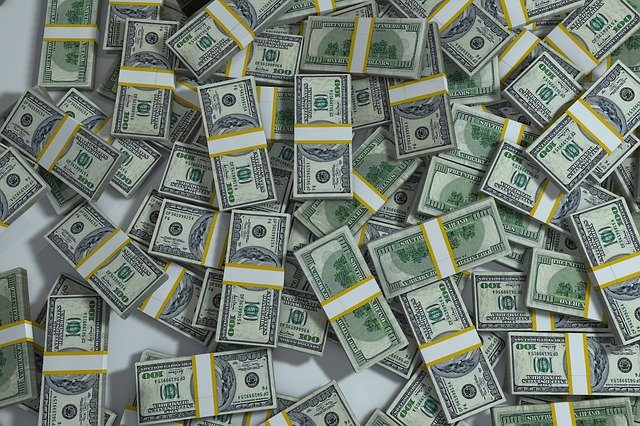
\includegraphics[width=0.5\textwidth]{cashStack}
\end{center}

For us as individuals, \$1,000,000,000 is certainly an eye-catching number, but that ad was trying to take advantage of how difficult it is to comprehend such large numbers.  Once again, though, we can put this amount in context by asking the question, ``what percentage of all taxes is this?''

In 2019, the U.S. federal government collected a total of \$3.5 trillion.  If we divide \$1 billion by this total, we find out that the billion dollars represents less than 0.03\% of all taxes collected, which is completely insignificant.

It turns out that there's an added benefit to calculating this percentage.  Once we know that number, we can use it to estimate how much an individual ``left behind,'' to borrow the terminology of the ad.  If someone paid \$10,000 in federal taxes, for instance, we can calculate 0.03\% of \$10,000.  We'll discuss how to do this more later, but it turns out that this is a grand total of\ldots around \$3.

Is that significant?  Maybe, or maybe not, but remember that this was part of an ad designed to sell accounting services, and it seems unlikely they'd charge less than \$3 for their services.

\subsection{Word Problems with Percentages}
Consider the following three questions (you don't need to solve them yet; just look at their structure).
\begin{itemize}
\item What is 20\% of 275?
\item Eighteen is what percentage of 54?
\item Twelve is 45.3\% of what?
\end{itemize}

Do you notice any similarities?  If you look carefully, you should see a common structure.

\begin{formula}{Applied Percentage Problems}
Every applied percentage problem can be written in the following form:
\begin{center}
$A$ is $P$ percent of $B$
\end{center}
Remember that when translating a sentence into its mathematical form, the word ``is'' gets replaced with the equals sign (since ``is'' really means ``this thing and that thing are equal''), and the word ``of'' gets replaced with multiplication.

This means that every percentage problem is built around the equation
\[A = PB\]
and in every problem, two of these pieces are given, and we simply have to solve for the missing piece.
\end{formula}

If you'd like, you can use the equation above every time, substituting the appropriate values each time.  The examples we started with would look like this, for instance:
\begin{itemize}
\item $A = (20\%)(275)$
\item $18 = (P)(54)$
\item $12 = (45.3\%)(B)$
\end{itemize}

However, in order to solve these problems in a more general way, we'll use $x$ to represent the unknown piece each time.  This means that for our examples, we would write
\begin{itemize}
\item $x = (20\%)(275)$
\item $18 = (x)(54)$
\item $12 = (45.3\%)(x)$
\end{itemize}

The reason for this is that once you get used to translating a word problem into its mathematical form and replacing the unknown with $x$, you can take that process and apply it to other kinds of problems.

\begin{proc}{Percentages or Decimals?}
Remember that a percentage is simply another way to express a decimal or fraction (50\% is the same as 0.5, which is also the same as 1/2).

It's important to remember that percentages are just meant for displaying numbers, not for doing calculations.

\begin{center}
\textbf{When doing calculations, always use the decimal form of a percentage.}
\end{center}

As you'll see in many of the examples to follow, we'll give answers in both decimal form and percentage form, so you should be comfortable converting back and forth.  It's common to give an answer in the same form as the problem is given, though, so if someone asks you a question about a percentage, you should give your answer as a percentage, even though you'll use decimals during the calculation phase.
\end{proc}

\begin{example}{Setting up Percentage Questions}
Answer each of the following questions:
\begin{enumerate}[(a)]
\item What is 75\% of 690?
\item Forty is what percentage of 150?
\item Eight is 62\% of what?
\end{enumerate}

\sol
Just like we did at the start of the section, we'll start by rewriting each of these as an equation, with $x$ in place of the word ``what.''  Then we simply need to solve for $x$; be careful, though, to note whether $x$ represents a percentage or not, so that we know how to phrase the answer.

\begin{enumerate}[(a)]
\item What is 75\% of 690?
\[x = (75\%)(690)\]
This equation is already solved for us, in the sense that $x$ is already alone on one side; all that we have to do is calculate 75\% times 690, and we're done.  However, we need to remember:
\begin{center}
\textbf{When doing calculations, always use the decimal form of a percentage.}
\end{center}
That means that we need to rewrite 75\% as a decimal; remember that to do this, we simply divide 75 by 100 (or drop the percentage symbol and move the decimal place two places to the left).
\begin{align*}
75\% &= \dfrac{75}{100} = 0.75\\
x &= (0.75)(690)\\
&= \boxed{517.5}
\end{align*}
\pagebreak

\item Forty is what percentage of 150?
\[40 = (x)(150)\]
To solve for $x$, we need to get rid of the 150 that is multiplied onto it; we do this by dividing both sides by 150:
\begin{align*}
40 &= (x)(150)\\
\dfrac{40}{150} &= x\\
0.2667 &= x
\end{align*}
Notice that at the end of the calculation, we have the answer as a decimal, but since the question asked ``what \emph{percentage}...'' we should give the answer as a percentage (multiply by 100 and add the percentage symbol):
\[x = \boxed{26.67\%}\]

\item Eight is 62\% of what?
\[8 = (62\%)(x)\]
Again, start by rewriting 62\% as a decimal, then solve for $x$ by dividing both sides of the equation by the result.
\begin{align*}
8 &= (0.62)(x)\\
\dfrac{8}{0.62} &= x\\
\boxed{12.9} &= x
\end{align*}
\end{enumerate}
\end{example}

\begin{try}
Answer each of the following questions:
\begin{enumerate}[(a)]
\item What is 20\% of 275?
\item Eighteen is what percentage of 54?
\item Twelve is 45.3\% of what?
\end{enumerate}
\end{try}

Here's the good news: if you can do those three examples, there's no problem in this section you can't solve.  Every single word problem involving percentages follows the pattern of one of those three; all you have to do is figure out which pattern it is.\\

For instance, if you find that you paid \$4000 in federal income tax one year on a salary of \$45,662, you can figure out your \emph{effective tax rate}, meaning what percentage of your income went to income tax.  Just rephrase this in the standard form; what you really want to know is
\begin{center}
\$4000 is what percentage of \$45,662?
\end{center}
Once you see it in that form, you can run through the same steps as the last example, and you'll soon see that to get the answer, you'll need to divide \$4000 by \$45,662.

It may be that you eventually get to the point where you can simply get used to jumping to that step and skipping the rest of the process.  If you do, feel free to do so, but if you're not comfortable skipping steps, you can always deliberately set up the problem in this standard form.
\vfill
\pagebreak

\begin{example}[https://www.youtube.com/watch?v=cApv0GeF2XM]{Coffee Survey}
The Frederick News Post did a poll of 1500 people, asking them the following question: ``Do you go to Starbucks at least 3 times a week?'' Of those 1500 polled, 58\% said ``yes.''  How many people replied yes to the survey?

\sol
The goal is to rephrase this question in a familiar form, along the lines of 
\begin{center}
$A$ is $P$ percent of $B$
\end{center}
and figure out where the ``what'' goes (which part of the problem is unknown).\\

We know there are a total of 1500 people surveyed, and we know that \textbf{of} that total, 58\% responded ``yes.''  This means that our question looks like
\begin{center}
What is 58\% of 1500?
\end{center}

If we replace ``is'' with the equals sign and ``of'' with multiplication, we get the following equation:
\begin{align*}
x &= (58\%)(1500)\\
&= (0.58)(1500)\\
&= \boxed{870}
\end{align*}

Thus, 870 people responded ``yes'' to the survey.
\end{example}

\begin{try}[http://izzomath.com/103text/finance/example1.4/story.html]
If there are 6,233 students enrolled this semester, and 59\% of those are women, how many women are attending the college this semester?
\end{try}

Let's try one with the shortcut: rather than setting up the full equation and solving for $x$, remember that if we're looking for a percentage, it's going to be one number divided by the other.  Here's the trick: if you can't figure out which order to use for division, try one and see if your answer is on the right side of 100\%.

In other words, say your question is ``Five is what percentage of 10?''  If you divide 10 by 5, you get 10/5 = 2, which is equal to 200\%.  Since this is greater than 100\%, this answer claims that 5 is greater than 10, so clearly that's the wrong order for division.  If we go back and divide 5 by 10, we'll get the correct answer.

Of course, after you do this a few times, you'll get used to the idea that the number by itself on one side of the ``is'' gets divided by the number that's mentioned with the percentage.

\begin{example}[https://www.youtube.com/watch?v=1GTPRROi1tE]{Dog People}
\marginnote{
\includegraphics[scale=0.15]{Puppy1}}
In a survey of 400 people, 243 responded that they like dogs.  What percentage of these people like dogs?

\solline

Let's try the shortcut method here.  The question can be rephrased ``What percentage of 400 is 243?''  We know, since we're looking for the percentage, that we need to divide these two numbers, but the only question is what order to use for the division.\\

If we divide 400 by 243, we'll get a number larger than 1, or a percentage greater than 100\%, which can't be right, so we need to divide 243 by 400:

\[=\dfrac{243}{400} = 0.6075 = \boxed{60.75\%}\]

Roughly 61\% of people responded that they like dogs.
\end{example}

\begin{try}[http://izzomath.com/103text/finance/example1.3/story.html]
Three of the nine sitting members of the U.S. Supreme Court are female.  What percentage of the court is comprised of women?
\end{try}
\pagebreak

\text{}
\vfill

\begin{proc}{Tips for Percentage Problems}
In the standard problem
\begin{center}
$A$ is $P$ percent of $B$
\end{center}
there are three possibilities for what to solve for: $A$, $P$, and $B$.
\begin{itemize}
\item To solve for the percentage $P$, you'll always need to divide one of the given numbers by the other.  To find the order of division, think about whether the answer should be greater than or less than 1 (or 100\%).  If it should be greater than 1, divide the larger number by the smaller one, and vice versa.
\begin{itemize}
\item \textbf{Note:} the number by itself on one side of the word ``is'' will be divided by the other
\end{itemize}
\item If the percentage is given, and the goal is to find $A$ or $B$, you'll need to either multiply or divide the given number by the percentage that's given.  Which one you do depends on which number you're given:
\begin{itemize}
\item If you know the number that's linked to the percentage by the word ``of,'' multiply, since ``of'' is equivalent to multiplication.
\item Otherwise, divide the given number by the percentage.
\end{itemize}
\end{itemize}
\end{proc}
\vfill

\begin{example}[https://www.youtube.com/watch?v=cApv0GeF2XM]{Sales Tax}
Suppose that you load a grocery cart with \$159 worth of groceries, and the local sales tax rate is 7\%. How much tax do you pay, and what is the total cost of the groceries?\\

\sol
The sales tax rate tells you what percentage of the price will be added on top, so we'll calculate 7\% of \$159 and add that to \$159:
\begin{align*}
(\$159)(7\%) = (\$159)(0.07) &= \$11.13\\
&+ \$159 = \boxed{\$170.13}
\end{align*}

\marginnote{\bfseries Alternate Solution}
We could simplify the solution by noticing that we start with 100\% of the cost and add 7\% to it, so we end up with 107\% of the cost: \[(\$159)(107\%) = (\$159)(1.07) = \$170.13\]
\end{example}
\vfill

Taxes are not much fun to think about, so let's switch briefly to the happier side: discounts.  When you go to a store that advertises a sale of 30\% off, that means that whatever price is on the sticker will get 30\% slashed.  Just like before, we can calculate the new price by finding 30\% of the sticker price and subtracting that.  Alternately, we could notice that if we're removing 30\% of the price, we'll be left with 70\% of the price.  The next example illustrates a similar situation.
\vfill
\text{}
\pagebreak

\begin{example}{Discount}
\marginnote{
\includegraphics[scale=0.1]{TV1}}
For months you have been wanting a 47'' LCD flat screen television, but the price has been too high. The store is having a one-day sale on all televisions in the store. For one day only you can take 25\% off any television. The regular price on the television
you want is \$1099.
\begin{enumerate}[(a)]
\item What is the sale price?
\item What will the final price, including sales tax, be if the sales tax rate is 8\%?
\end{enumerate}

\solline
\begin{enumerate}[(a)]
\item Since the sale takes 25\% off the top of the price, the sale price will be 75\% of the original price:
\begin{align*}
\textrm{Sale price } &= (75\%)(\$1099)\\
&= (0.75)(\$1099)\\
&= \boxed{\$824.25}
\end{align*}

\item To add the sales tax, add 8\% to this new price, so we can find 108\% of \$824.25:
\begin{align*}
\textrm{Final price } &= (108\%)(\$824.25)\\
&= (1.08)(\$824.25)\\
&= \boxed{\$890.19}
\end{align*}
\end{enumerate}
\end{example}

\begin{try}[http://izzomath.com/103text/finance/example1.6/story.html]
You have a 20\% off coupon at Bed, Bath, and Beyond, and you're ready to get some new towels.  If you select some that are listed at \$30, and sales tax is 6\%, how much will your final cost be at the register?  Note that the discount is applied \textbf{before} the sales tax.
\end{try}

\paragraph{WATCH OUT!} There's a subtle pitfall lurking in the last example: you may think that since we're removing 25\% of the price for the sale, and adding 8\% for the tax, we could simple combine everything into one step and simply remove 17\% (the difference between 25\% and 8\%).

But that's not right, and if you try that calculation, you'll find that you get a different answer.  What happened?  It may be hard to spot at first, but notice that the sale is 25\% \emph{of the original price} and the tax is 8\% \emph{of the reduced price}.  Since these percentages are tied to \textbf{different} bases, they can't be combined.

This is an important idea, because this error is an easy one to see.  In fact, once you understand this, you'll likely spot this mistake in all sorts of places.

\begin{example}[https://www.youtube.com/watch?v=14sOMJuqxrA]{A Tricky Percentage Problem}
Suppose you originally paid \$1200 in taxes.  A year later taxes decreased by 20\%, but the following year taxes increased by 20\%.  What do you pay in taxes at the end?

\sol

You may be tempted to jump to the conclusion that you'll pay \$1200 in taxes at the end, since the 20\% decrease was reversed by the 20\% increase.  Be careful, though: the decrease was 20\% of \emph{the original amount} and the increase was 20\% of \emph{the reduced amount}.  Thus, the increase was \emph{smaller} than the increase, so we expect to pay less than \$1200 at the end.\\

Specifically, after one year, the taxes would be \[(\$1200)(0.80) = \$960.\]  After two years, the taxes would be \[(\$960)(1.20) = \boxed{\$1152}\]
\end{example}

\subsection{Percentage Increase or Decrease}
There's another kind of problem involving percentages: we can talk about \textbf{percentage change}.  For instance, you might hear a presidential candidate promise to cut taxes by 12\%, or you may hear that there are 25\% more hurricanes one year than the year before.

Of course, there's no such thing as a \emph{new} percentage problem, because we know that every percentage problem has to fall into one of three categories, and we've done examples of all three.  Our only job, then, is to find how to use what we already know to solve these problems that are stated a bit differently.

The most important thing to keep in mind with a percentage change problem is
\begin{center}
The change is given as a percentage \textbf{of the \emph{original} amount}
\end{center}

For instance, if you knew that there were originally 400 employees at a company, and 30 of them were laid off, this means that the size of the workforce decreased by whatever percentage 30 is of 400, so the problem boils down to ``Thirty is what percentage of 400?''  Having solved several problems of that type, we know to divide 30 by 400, and that leads to the following formula.

\begin{formula}{Percentage Change}
The percentage change, or relative change, of a quantity is defined as the ratio of the total change to the original amount:
\[\textrm{Percentage Change } = \dfrac{\textrm{Total Change}}{\textrm{Original Amount}}\]
where the Total Change is the difference between the final and original amounts:
\[\textrm{Total Change} = \textrm{Final Amount} - \textrm{Original Amount}\]

If the percentage change is positive, the quantity increased; if it is negative, the quantity decreased.
\end{formula}

As long as you don't forget to divide by the \textbf{original amount}, not the final amount, these problems are straightforward.

\begin{example}[https://www.youtube.com/watch?v=gH7XJFdMsRc]{Car Value}
\marginnote{
\includegraphics[scale=0.1]{Car1}}
The value of a car dropped from \$7400 to \$6800 over the last year. What percentage decrease is this?

\solline

First, find the absolute change:
\[\$7400 - \$6800 = \$600\]
Then divide this by the \textbf{original amount}:
\[\dfrac{\$600}{\$7400} = 0.081 = \boxed{8.1\%}\]

Thus, the value of the car dropped by 8.1\%.
\end{example}

\begin{try}[http://izzomath.com/103text/finance/example1.7/story.html]
You go car shopping and find your dream car for \$11,000 sitting on the lot, but unfortunately you only have \$9,000 to pay for it.  You offer the dealership the money you have and they accept your offer.  What percentage did the dealership take off the car?
\end{try}

We can also turn this kind of problem around: if we know the percentage change, we can find either the original or final amount.

If we know the original amount and the percentage change, this is exactly like the problems with discounts and sales taxes from earlier; we have a starting value and a percentage adjustment, and need to find the final amount.

Going in the other direction is a bit trickier: to find the original amount when we know the final amount and the percentage change, we need to think carefully, because the change is given as a percentage of the \emph{unknown} value.

\begin{example}{Amount Before an Increase}
\marginnote{
\includegraphics[scale=0.08]{Books1}}
If the tuition and fees paid by the average student in the U.S. is \$9,139, and this is 17\% more than the average five years ago, what was the average cost then?

\solline

The new amount---\$9,139---is 117\% of the original cost.  Since we don't know what the original cost was, we need a placeholder for it, so we'll call it $x$:
\[\$9,139 = (117\%)(x)\]
\begin{align*}
x &= \dfrac{\$9,139}{117\%}\\
&= \dfrac{\$9,139}{1.17}\\
&= \boxed{\$7,811}
\end{align*}
The original cost, then, was \$7,811 for the average student five years ago.
\end{example}

Relative change or percent differences are also useful when comparing quantities of different sizes.  By calculating the percent difference, we can put everything on equal footing to make a meaningful comparison.

\begin{example}[https://www.youtube.com/watch?v=Bhqb1XOWcQQ]{Enrollment Changes}
Generally, more students go to college every semester than the semester before.  In the fall semester of 2008 there were 5,748 students enrolled at FCC; by the fall of 2009, the number had grown to 6,233.  Compare these two numbers.

\sol
We could compare them by simply finding the difference, and saying that there were 485 more students in 2009 than in 2008, but out of context this number is mostly meaningless.  At a small school like FCC, this may represent a dramatic change, but at a larger school like the author's alma mater of North Carolina State, 485 students wouldn't be as significant.\\

Instead, we can calculate this as a percentage change:
\[\dfrac{485}{5748} = 0.084 = 8.4\%\]
Enrollment rose by 8.4\%, which is a modest but respectable gain.
\end{example}

\begin{try}
If you took the SAT twice, scoring 500 on the verbal portion the first time and 620 the second time, by what percentage did your score increase?
\end{try}
\pagebreak

This idea of putting different quantities on equal footing in order to compare them is extremely powerful, and crucial in many contexts.  We'll do something similar later when we consider financial applications; there, we'll be interested in, for instance, comparing two loans with different interest rates and durations and deciding which is more advantageous.  The details will differ, but the concept of finding common ground on which to compare different quantities comes up in many areas.

\begin{example}{Comparisons}
There are 435 Longhorn Steakhouse locations in the U.S. and 136 Ruth's Chris Steakhouse locations.  Compare these two numbers.

\sol
Rather than simply saying that there are 299 more Longhorn locations that Ruth's Chris, let's use a meaningful measure like the percentage difference.\\

We could say that Longhorn is $\frac{299}{136} = 219.9\%$ larger, or that Ruth's Chris is $\frac{299}{435} = 68.7\%$ smaller.  We could also say that Ruth's Chris is $\frac{136}{435} = 31.3\%$ of the size of Longhorn.
\end{example}

We've solved a wide array of problems using percentages, but every problem fit into one of the three categories introduced at the beginning of the section.  In the next section, we'll apply these skills to calculate how interest accrues for different kinds of loans.